\section{The P\'olya route}\label{ch:polya}

P\'olya's integral \eqref{eq:ch2:mgf} evaluates $\xi$ in the complex plane from the kernel alone, without primes or zeros. In this chapter, $\delta$ always denotes the distance from the line of integration to the edge of the strip of analyticity of $\Phi$, not the displacement of an off line zero.

\subsection{The trapezoid rule on P\'olya's integral}\label{sec:ch4:trapezoid}

Recall the P\'olya kernel \eqref{eq:ch2:Phi} in Titchmarsh's normalisation \cite[Section 10.1]{Titchmarsh},
\begin{equation}\label{eq:Phi}
\Phi(u)=2\sum_{n\ge1}\big(2\pi^2n^4e^{9u/2}-3\pi n^2e^{5u/2}\big)\exp(-\pi n^2e^{2u}),
\end{equation}
even and positive on the real line, analytic in the strip $|\im u|<\pi/4$ (Section~\ref{ch:clock}) and doubly exponentially decaying in every closed substrip (proof of Proposition~\ref{prop:tilt}). With the P\'olya variable $X$ of density $p=\Phi/\Xi(0)$, the moment generating function \eqref{eq:ch2:mgf} and its derivative under the integral sign give, for every complex $s$,
\begin{equation}\label{eq:xi}
\frac{\xi(\tfrac12+s)}{\xi(\tfrac12)}=\E\,e^{sX}=\E\cosh(sX),\qquad \frac{\xi'(\tfrac12+s)}{\xi(\tfrac12)}=\E\,Xe^{sX},\qquad X\sim p,
\end{equation}
so the Thorin density \eqref{eq:rho} is $\pi^{-1}\re\{\E Xe^{sX}/\E e^{sX}\}$ at $s=\varepsilon+i\theta$. Throughout, $\log$ is the natural logarithm.

Analyticity and decay in the strip make the trapezoid rule with nodes $u_j=jh$ converge geometrically in $1/h$ \cite[Theorem 5.1]{TW14} (Exercise~\ref{ex:ch4:trapezoid}): for $s=\varepsilon+i\theta$,
\[
\Big|\int_{\R}\Phi(u)e^{su}\,du-h\sum_{j\in\mathbb Z}\Phi(jh)e^{sjh}\Big|\le \frac{2K_\eta(\varepsilon)\,e^{\eta|\theta|}}{e^{2\pi\eta/h}-1},\qquad 0<\eta<\pi/4,
\]
where $K_\eta(\varepsilon)=\int_{\R}|\Phi(x\pm i\eta)|\,e^{\varepsilon|x|}\,dx$, the same for both signs because $\Phi$ is real on the real axis. We write $K_\eta=K_\eta(0)$. Since $|\xi(\tfrac12+\varepsilon+i\theta)|$ decays like $e^{-\pi\theta/4}$, the relative error is at most of order $\exp\{(\eta+\pi/4)\theta-2\pi\eta/h\}$. With $h=1/200$ the bound is best for $\eta$ close to $\pi/4$, and at $\theta=200$ it is about $10^{-289}$; halving $h$ changes the computed values by less than $10^{-64}$.

The limit in practice is the cancellation in \eqref{eq:xi}: the integrand is of order one and the integral of order $e^{-\pi\theta/4}$, so at $b$ bits the rounding error is of order $2^{-b}e^{\pi\theta/4}$ relative to $|\xi|$, a loss of $\pi\theta/(4\log10)=0.341\,\theta$ decimal digits. Discretisation, rounding and the truncation of the $u$ axis at $|u|\le L$ can be budgeted separately. To reach $D$ correct digits at height $\theta$ one needs
\[
b\ \ge\ \Big(D+\frac{\pi\theta}{4\log10}\Big)\log_2 10,\qquad h\ \le\ \frac{2\pi\eta}{(D+0.682\,\theta)\log10},
\]
where the condition on $h$ uses $\eta+\pi/4\le\pi/2$. The truncation needs $\pi e^{2L}\ge(D+0.341\,\theta)\log10+|\varepsilon|L$, up to lower order terms.

We take $h=1/200$ and $L=3$, beyond which $\Phi$ is below $10^{-500}$, and work at $420$ bits ($126$ decimal digits): at height $200$, where $|\xi|$ is about $10^{-63}$, the cancellation consumes about half of them and leaves about $60$. Truncating the sum at $|j|\le J=L/h$ and folding it with the evenness of $\Phi$ gives, with $E=e^{sh}$,
\[
\xi(\tfrac12+s)\approx P(E)+P(E^{-1}),\qquad \xi'(\tfrac12+s)\approx Q(E)-Q(E^{-1}),
\]
\[
P(x)=\tfrac h2\Phi_0+h\sum_{j=1}^{J}\Phi_jx^j,\quad Q(x)=h^2\sum_{j=1}^{J}j\Phi_jx^j,
\]
with $\Phi_j=\Phi(jh)$ and $J=600$. The node values, the only place where the theta series is summed, are computed once for a given step, truncation and precision and serve every resolution and every height; one evaluation of $\xi$ and $\xi'$ then costs four polynomial evaluations in ball arithmetic \cite{Arb}, about $0.7$ ms at $420$ bits. The ball radii certify the rounding error only, and they overestimate it: at height $200$ they certify about $38$ digits of $\xi$ and, at $\varepsilon=0.005$, about $36$ of $\re(\xi'/\xi)$, while comparison with \texttt{mpmath} at $90$ digits shows that the values themselves carry about $63$.

\subsection{Zeros and Thorin masses below height 200}\label{sec:ch4:height200}

With the parameters of Section~\ref{sec:ch4:trapezoid}, the zeros and the Thorin masses below height $\Theta=200$ are computed at the eight resolutions $\varepsilon=1,\allowbreak0.5,\allowbreak0.25,\allowbreak0.1,\allowbreak0.05,\allowbreak0.02,\allowbreak0.01,\allowbreak0.005$ in five steps.
\begin{enumerate}
\item Compute $\Phi_j$, $0\le j\le J$, from \eqref{eq:Phi} at $420$ bits.
\item For each resolution $\varepsilon$, evaluate $\rho_\varepsilon(\theta_k)$ and $M_\varepsilon(\theta_k)=\pi^{-1}\arg\xi(\tfrac12+\varepsilon+i\theta_k)$, with the branch of the argument that vanishes at $\theta=0$, on the grid $\theta_k=k\varepsilon/8$ ($k\varepsilon/4$ at $\varepsilon=0.005$), $0\le\theta_k\le\Theta$. Since $\partial_\theta\arg\xi(\alpha+i\theta)=v_\alpha(\theta)$ with $\alpha=\tfrac12+\varepsilon$, $M_\varepsilon(\theta)=\mu_\varepsilon((0,\theta^2])$ is exactly the cumulative Thorin mass.
\item Locate the line zeros as sign changes of $\Xi(\theta)=\xi(\tfrac12+i\theta)$ on a grid of step $0.05$, reading each sign from a ball that excludes zero, and refine them by Newton's method using $\Xi'(\theta)=-\im\xi'(\tfrac12+i\theta)$.
\item Count all zeros with $0<\im\rho\le\Theta$ by the argument principle, $N(\Theta)=\pi^{-1}\Delta\arg\xi(s)$ along $2\to2+i\Theta\to\tfrac12+i\Theta$ \cite[Section 9.3]{Titchmarsh}.
\item Compare with $U_{\RH}$ in the metrics of Section~\ref{ch:distances}.
\end{enumerate}
Steps 3 and 4, which use the same two polynomials, together bound the number of off line zeros. Each sign change of $\Xi$ on the grid encloses at least one zero on the line, so $N(\Theta)$ minus the number of sign changes is an upper bound for the number of off line zeros with $0<\im\rho\le\Theta$. When the two numbers agree, every zero below height $\Theta$ is on the line and simple.

In step 2 the argument is accumulated from the increments $\arg(\xi(s_{k+1})/\xi(s_k))$ along $\re s=\frac12+\varepsilon$. The principal value is the true increment only if $\arg\xi$ changes by less than $\pi$ between consecutive points, which the samples cannot show; the grids are chosen so that every observed increment is below $\pi/2$ in modulus, a margin checked after the fact rather than a guarantee, and the largest observed was $0.29$. At large height $\xi$ underflows double precision ($|\xi|$ is about $10^{-335}$ at height $1000$), so the quotient must be formed in ball arithmetic before the argument is taken.

With $\Theta=200$ there are $79$ sign changes, and at none of the $4001$ grid points does the ball for $\Xi$ contain zero. The argument principle gives $N(200)=79.0000000000004$, with a largest increment of $0.02$ radians along the contour, and $\Theta=200$ lies between $\gamma_{79}=198.0153$ and $\gamma_{80}=201.2648$, so it is not an ordinate. The Newton refined roots agree to $5.0\times10^{-48}$ with the ordinates computed independently by \texttt{mpmath} \cite{mpmath} at $50$ digits. The computation thus recovers, with no input but \eqref{eq:Phi}, the classical fact that the $79$ zeros below height $200$ lie on the line and are simple \cite{Backlund,PT21}. It is not yet a proof: the argument increments are summed in double precision from samples, and the analytic error bounds are not added to the radii (Section~\ref{st:sec:wp2} lists what a certified version requires). Figure~\ref{fig:density} shows the computed density.

\begin{figure}[t]
\centering
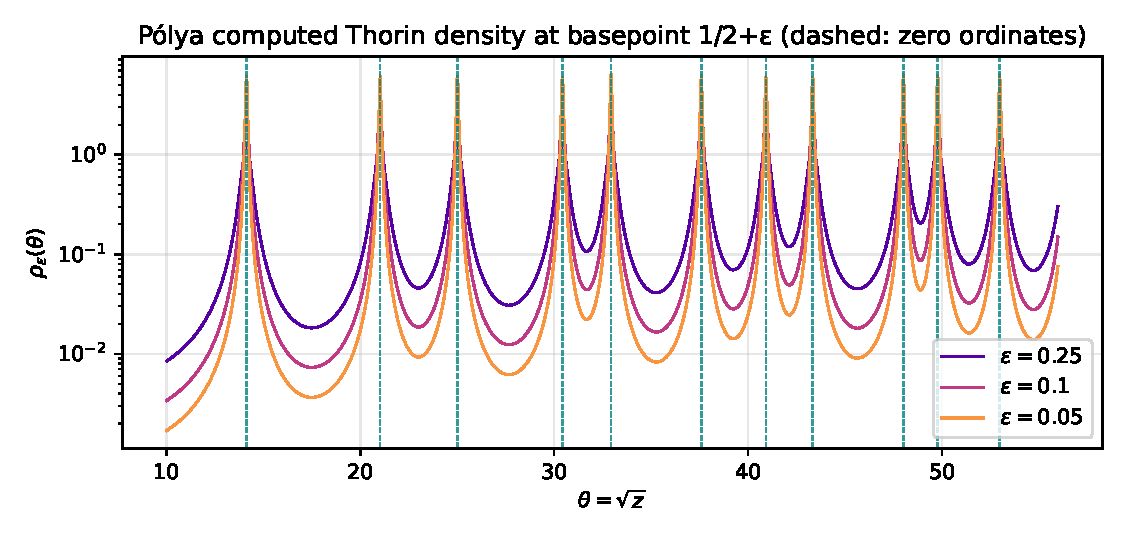
\includegraphics[width=0.95\textwidth]{fig/density.pdf}
\caption{The Thorin density $\rho_\varepsilon(\theta)$ at basepoint $\tfrac12+\varepsilon$ computed from the P\'olya density, for $\varepsilon=0.25,0.1,0.05$ and $10<\theta<56$, on a logarithmic scale; dashed lines mark the ordinates. Each ordinate carries a Cauchy kernel of height $1/(\pi\varepsilon)$ and mass one (Proposition~\ref{prop:struct}).}
\label{fig:density}
\end{figure}

\subsection{Tilting the contour into the strip}\label{sec:newcomp}

Since $\Phi$ is analytic in $|\im u|<\pi/4$, the integrals behind \eqref{eq:xi} can be taken along any horizontal line inside the strip.

\begin{proposition}\label{prop:tilt}
Let $0<\delta<\pi/4$ and $\eta=\pi/4-\delta$. For every complex $s$,
\begin{align*}
\xi\Big(\frac12+s\Big)&=e^{i\eta s}\int_{\R}\Phi(x+i\eta)\,e^{sx}\,dx,\\
\xi'\Big(\frac12+s\Big)&=e^{i\eta s}\int_{\R}(x+i\eta)\,\Phi(x+i\eta)\,e^{sx}\,dx .
\end{align*}
For real $x$, $|\Phi(x+i\eta)|\le C_\delta$ and $|(x+i\eta)\Phi(x+i\eta)|\le C_\delta$, with $C_\delta=O(\delta^{-5/2})$ as $\delta\to0$.
\end{proposition}

\begin{proof}
By Section~\ref{ch:clock}, $\Phi$ is analytic in $|\im u|<\pi/4$, and by the identity theorem its evenness $\Phi(u)=\Phi(-u)$ extends from the real line to the strip. For $u=x+iy$ with $|y|\le\eta$ and $x\ge0$ we have $\re e^{2u}=e^{2x}\cos2y\ge e^{2x}\sin2\delta$, so
\begin{equation}\label{eq:ch4:majorant}
|\Phi(x+iy)|\le2\sum_{n\ge1}\big(2\pi^2n^4e^{9x/2}+3\pi n^2e^{5x/2}\big)\exp(-\pi n^2e^{2x}\sin2\delta),
\end{equation}
and $\Phi$ decays doubly exponentially as $x\to+\infty$, uniformly in the closed strip $|y|\le\eta$; by evenness it does so as $x\to-\infty$ as well. Cauchy's theorem therefore moves the line of integration in $\xi(\tfrac12+s)=\int_{\R}\Phi(u)e^{su}\,du$, which is \eqref{eq:xi}, from $\im u=0$ to $\im u=\eta$, and the second identity follows in the same way from $\xi'(\tfrac12+s)=\int_{\R}u\Phi(u)e^{su}\,du$. Finally, $\sum_{n\ge1}n^ke^{-bn^2}=O(b^{-(k+1)/2})$ uniformly in $b>0$, so the majorant \eqref{eq:ch4:majorant} is $O(e^{-x/2}\delta^{-5/2})$ for $x\ge0$, of order $\delta^{-5/2}$ at $x=0$; with evenness this gives both bounds.
\end{proof}

On the real axis the integrand $\Phi(u)e^{su}$, with $s=\varepsilon+i\theta$, oscillates with frequency $\theta$, and its integral, of order $\theta^{7/4+\varepsilon/2}e^{-\pi\theta/4}|\zeta(\tfrac12+\varepsilon+i\theta)|$ by Stirling's formula, is exponentially smaller than the integrand. On the line $\im u=\eta$ the factor $e^{i\theta u}$ has constant modulus $e^{-\theta\eta}$ and leaves the integral as the prefactor $e^{i\eta s}$, which carries almost all of the decay of $\xi$; the integral that remains is of order $e^{-\delta\theta}$ up to the same factors, against an integrand of size at most $C_\delta e^{\varepsilon x}$. The cancellation thus drops from $e^{-\pi\theta/4}$ to $e^{-\delta\theta}$. The price is a larger kernel, by the factor $K_\eta/K_0$ with $K_0=\xi(\tfrac12)=0.497$, and a finer step, because the natural boundary at $\im u=\pi/4$ \cite[Chapter 11, Section 1.4, and Chapter 5, Section 3.2]{Remmert98} is now only $\delta$ away.

On the tilted line the kernel constant measures the size of the integrand and costs $\log_{10}K_\eta$ digits of precision. By Table~\ref{tab:ch4:Meta} it grows like $\delta^{-5/2}$, but $\log_{10}K_\eta$ stays under five even at $\delta=0.01$, which is negligible against the saving $(\pi/4-\delta)\theta/\log10$ at any height where tilting is worthwhile.

\begin{table}[htbp]
\centering\small
\begin{tabular}{rrr}
\toprule
$\delta=\pi/4-\eta$ & $K_\eta$ & $\max_x|\Phi(x+i\eta)|$\\
\midrule
0.6854 & 0.554 & 0.981\\
0.3927 & 2.52 & 3.24\\
0.2 & 19.0 & 15.4\\
0.1 & 126 & 76.5\\
0.05 & 774 & 415\\
0.02 & 7836 & 3938\\
0.01 & 43503 & 22207\\
\bottomrule
\end{tabular}
\caption{Size of the P\'olya kernel on lines inside its strip of analyticity, computed on a grid of step $0.002$ over $|x|\le6$; the first two rows are the lines $\eta=0.1$ and $\eta=\pi/8$. The growth is close to $\delta^{-5/2}$, as the majorant in the proof of Proposition~\ref{prop:tilt} predicts.}
\label{tab:ch4:Meta}
\end{table}

The trapezoid rule on the tilted line converges geometrically under two conditions (Exercise~\ref{ex:ch4:alias}). By Poisson summation its error is $\sum_{k\ne0}I(\theta+2\pi k/h)$, where $I(t)=\int_{\R}\Phi(x+i\eta)e^{\varepsilon x}e^{itx}\,dx=e^{\eta t-i\eta\varepsilon}\xi(\tfrac12+\varepsilon+it)$. The integrand is analytic in a strip that extends $\delta$ above the line and $\pi/2-\delta$ below it, and correspondingly $|I(t)|$ is of order $e^{-\delta t}$ as $t\to+\infty$ and $e^{-(\pi/2-\delta)|t|}$ as $t\to-\infty$, up to the factors of Stirling's formula. Relative to $I(\theta)$ the terms with $k\ge1$ are of order $e^{-2\pi\delta k/h}$, and those with $k\le-1$ are small only when the step resolves the oscillation $e^{i\theta x}$ with a margin. For $D$ correct digits this gives
\begin{equation}\label{eq:ch4:tiltcond}
\frac1h\ \ge\ \frac{D\log10}{2\pi\delta},\qquad \frac{2\pi}h\ \ge\ \theta+\frac{\delta\theta+D\log10}{\pi/2-\delta},
\end{equation}
up to terms of order $\log\theta+\log(1/h)$. The first condition asks for about $D\log10/(2\pi\delta)$ nodes per unit length, $458$ at $D=25$ and $\delta=0.02$, that is $h\le2.2\times10^{-3}$. The second is the binding one at large height: at $\delta=0.02$ and $25$ digits it is the stronger from about $\theta=2800$ on, and it asks for $h\le1.23\times10^{-3}$ at $\theta=5000$ and $h\le8.8\times10^{-4}$ at $\theta=7005$.

Taking $\delta$ proportional to $1/\theta$ holds the loss $\delta\theta/\log10$ fixed, so the working precision grows only through the $\log_{10}K_\eta$ digits of the kernel constant, about $\frac52\log_{10}(1/\delta)$, while both conditions \eqref{eq:ch4:tiltcond} make the number of nodes, and with it the cost per point, grow linearly in $\theta$ up to a logarithmic factor from the truncation.

\subsection{Precision and cost of the tilted route}\label{sec:ch4:budget}

The tilt makes height $5000$ accessible (Table~\ref{tab:tilt}).

\begin{table}[t]
\centering\small
\begin{tabular}{rrrrrrl}
\toprule
$\delta$ & bits & nodes & $\theta$ & error of $\xi'/\xi$ & ms per point & untilted digits needed\\
\midrule
0.10 & 200 & 2001 & 200 & $<2\times10^{-45}$ & 7 & 68\\
0.10 & 200 & 2001 & 500 & $9.8\times10^{-42}$ & 7 & 171\\
0.10 & 200 & 2001 & 1000 & $1.8\times10^{-20}$ & 7 & 341\\
0.02 & 220 & 8401 & 1000 & $<6\times10^{-45}$ & 28 & 341\\
0.02 & 220 & 8401 & 2000 & $<4\times10^{-45}$ & 28 & 682\\
0.02 & 220 & 8401 & 5000 & $2.9\times10^{-25}$ & 28 & 1705\\
\bottomrule
\end{tabular}
\caption{The tilted P\'olya route at $\varepsilon=0.05$, compared with \texttt{mpmath} at $50$ digits. Errors are absolute errors of $\xi'/\xi$, which bound those of its real part, and $<$ marks the entries at the floor set by rounding the tilted value to $45$ significant digits. The rows with $2001$ nodes use the step $h=0.004$ and the truncation $L=4$, those with $8401$ nodes $h=0.001$ and $L=4.2$. The last column is the number of digits, $0.341\,\theta$, that the untilted route loses to cancellation at the same height.}
\label{tab:tilt}
\end{table}

On the tilted line the rounding term of Section~\ref{sec:ch4:trapezoid} becomes $2^{-b}e^{\delta\theta}$ times the kernel constant, and the step obeys \eqref{eq:ch4:tiltcond}. Table~\ref{tab:ch4:budget} compares the working precision of the two routes. The formula of the table for the tilted bits is conservative: it ignores the factor $\theta^{7/4+\varepsilon/2}$ in $|\xi(\tfrac12+\varepsilon+i\theta)|$, worth about six digits at $\theta=5000$, and it adds five digits for the kernel constant. The run at $\theta=5000$ in Table~\ref{tab:tilt} used $220$ bits, fewer than the $244$ of Table~\ref{tab:ch4:budget}, and returned $25$ digits; the Lehmer pair of Section~\ref{sec:ch5:lehmer} was computed with $256$ bits at $\delta=0.01$, where the formula asks for $201$.

\begin{table}[htbp]
\centering\small
\begin{tabular}{rrrrr}
\toprule
height $\theta$ & target digits & bits (untilted) & bits (tilted, $\delta=0.02$) & nodes (tilted)\\
\midrule
100 & 30 & 213 & 119 & 8400\\
200 & 30 & 326 & 122 & 8400\\
1000 & 30 & 1233 & 145 & 8400\\
5000 & 25 & 5748 & 244 & 8400\\
7005 & 25 & 8020 & 302 & 8400\\
\bottomrule
\end{tabular}
\caption{Working precision needed by the untilted and the tilted P\'olya route for $D$ target digits. The untilted bits are $(D+\pi\theta/(4\log10))\log_210$ and the tilted bits $(D+\delta\theta/\log10+5)\log_210$, where the $5$ digits cover $\log_{10}K_\eta<5$ for $\delta\ge0.01$. At $\theta=7005$ the second condition in \eqref{eq:ch4:tiltcond} asks for $h\le8.8\times10^{-4}$, so $8400$ nodes give $25$ digits there only with a truncation near $|x|\le3.7$, the smallest that suffices.}
\label{tab:ch4:budget}
\end{table}

Because the tilt reduces the cancellation to $e^{-\delta\theta}$, ordinary double precision suffices at moderate height. With $\delta=0.15$ and the node values rounded to double, a vectorised evaluation agrees with the ball arithmetic values of $\rho_{0.05}$ to within an absolute error of $2.8\times10^{-12}$ for $\theta\le50$, $1.3\times10^{-9}$ for $\theta\le100$ and $7.6\times10^{-7}$ for $\theta\le150$, at $93\,\mu$s per point. The untilted route fails in double precision above $\theta\approx40$ (Exercise~\ref{ex:ch4:double}).



\subsection{Ball arithmetic on the tilted line}\label{sec:ch4:balls}

Horner's rule, which serves the untilted evaluator well, fails in ball arithmetic on the tilted line. The tilted evaluator writes the trapezoid sum as one polynomial of degree $2J$ in $E=e^{sh}$, with coefficients $h\Phi(x_k+i\eta)$ for $x_k$ running from $-L$ to $L$, times the prefactor $e^{i\eta s}E^{-J}$. With $2001$ nodes, $\delta=0.1$ and $200$ bits, the radius of the Horner recursion grew by a factor of about $1.3$ per step, and the final ball at $\theta=100$ had radius $10^{109}$ although its midpoint was correct to many digits. Evaluating each exponential $e^{sx_k}$ directly and summing gives balls of radius about $10^{-55}$ at the same point.

The cause is the wrapping effect of rectangular complex balls. Arb stores a complex number as a real ball and an imaginary ball \cite{Arb}, so a multiplication by $E=e^{\varepsilon h}e^{i\theta h}$ rotates the midpoint but multiplies the radii by $e^{\varepsilon h}(|\cos\theta h|+|\sin\theta h|)$, up to rounding; at $\theta h=0.4$ this factor is $1.31$. In Horner's rule the coefficient of $E^k$ passes through $k$ such multiplications. On the untilted line the effect is contained. The polynomials are folded at $x=0$, so the coefficient at $x=jh$ passes through at most $600$ multiplications, and the coefficients $h\Phi(jh)$ decay like $\exp(-\pi e^{2jh})$, so those that pass through many multiplications are negligible and the radii stay far below $|\xi|$ up to height $200$. On the tilted line the coefficients decay only like $\exp(-\pi e^{2x}\sin2\delta)$, and the coefficient at $x$ passes through $(x+L)/h$ multiplications. With $h=0.004$ and $L=4$, which give $2001$ nodes, the coefficients near $x=2$ are still of order $10^{-12}$ at $\delta=0.1$, and they pass through about $1500$ multiplications, which enlarge their radii by a factor of about $10^{176}$.
